\section{Case study}
\label{sec: case_study}


This section illustrates that RD-Gen can generate the random DAG sets used in the evaluation of existing studies based on DAGs.
Case studies of a single-rate DAG, a multi-rate DAG consisting of only timer-driven nodes, and a chain-based multi-rate DAG are shown, respectively.


\subsection{Case study 1}
\label{ssec: case_study_1}


\begin{figure*}[t]
    \begin{tabular}{c}
        %1
        \begin{minipage}{0.35\linewidth}
            \begin{flushleft}
                \begin{tabular}{l}
                    \lstset{linewidth=5.5cm, basicstyle=\scriptsize}
                    \lstinputlisting{src/code/case_study_single.txt}
                \end{tabular}
            \end{flushleft}
            \centering
            Input YAML file
        \end{minipage}
        % 2
        \begin{minipage}{0.22\linewidth}
            \centering
            \scalebox{1.0}{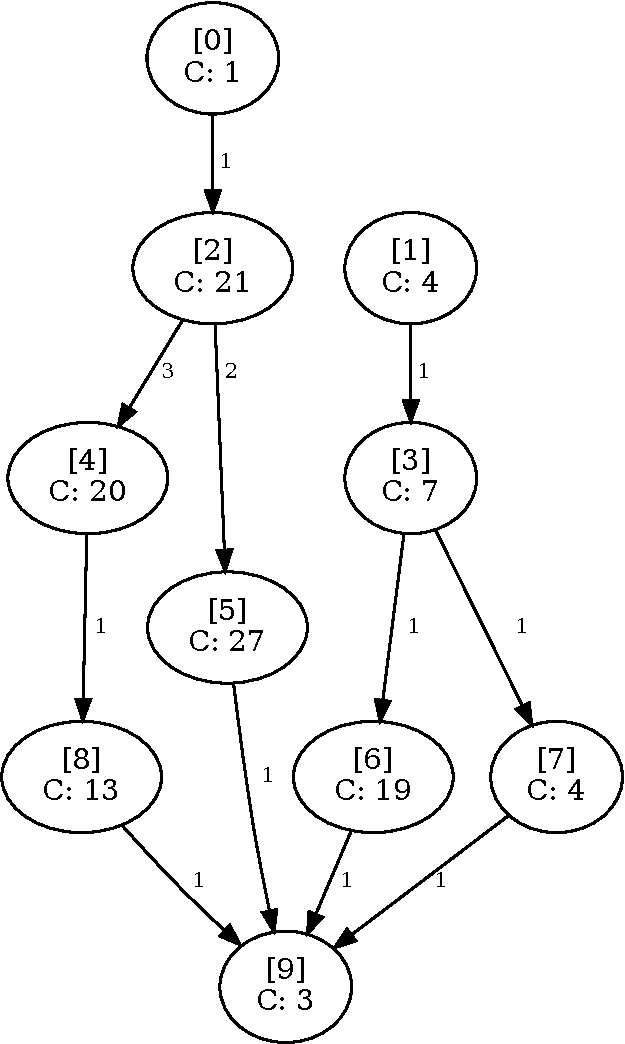
\includegraphics[keepaspectratio, width = \linewidth]{./src/figure/case_study_single/ccr_0.1.pdf}}
            \hspace{3.0cm} Number of nodes: 10, CCR: 0.1
        \end{minipage}
        % 3
        \begin{minipage}{0.47\linewidth}
            \centering
            \scalebox{0.8}{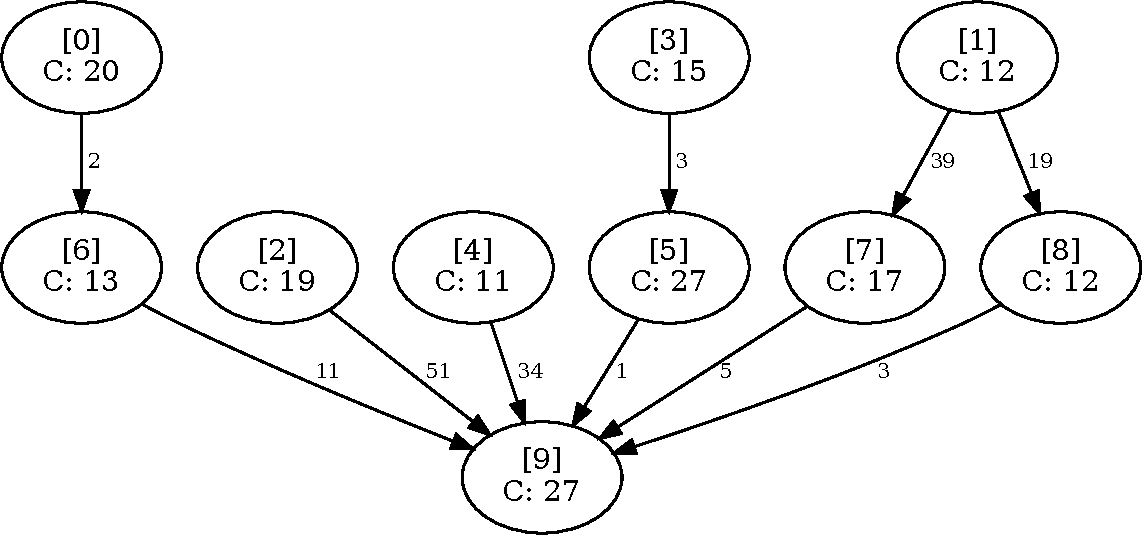
\includegraphics[keepaspectratio, width = \linewidth]{./src/figure/case_study_single/ccr_1.0.pdf}}
            \hspace{3.5cm} Number of nodes: 10, CCR: 1.0 \\
            \vspace{3mm}
            \centering
            \scalebox{0.7}{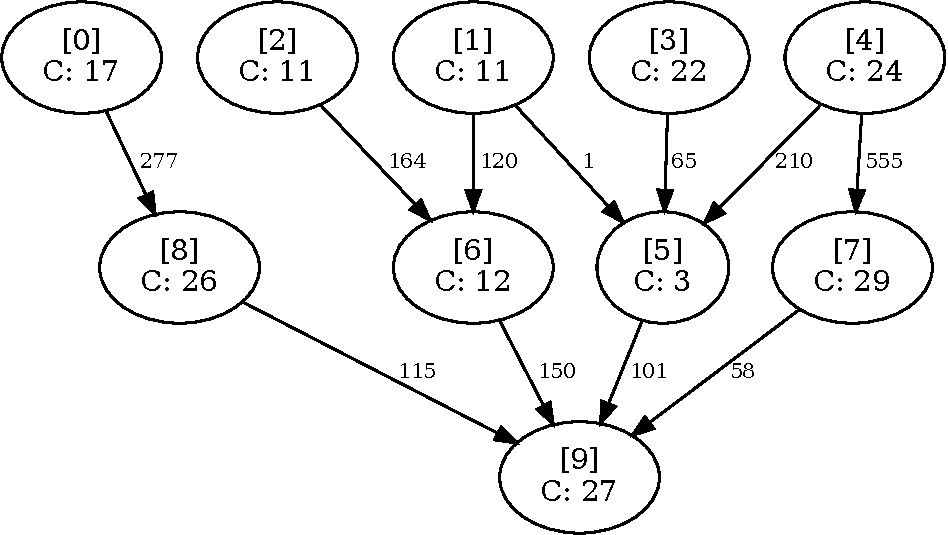
\includegraphics[keepaspectratio, width = \linewidth]{./src/figure/case_study_single/ccr_10.0.pdf}}
            \hspace{3.0cm} Number of nodes: 10, CCR: 10.0
        \end{minipage}
    \end{tabular}
    \centering
    \caption{Example of the generation a random DAG set with varying CCR, number of nodes, execution time, and communication time using the {\it Fan-in/Fan-out} method.}
    \label{fig: case_study_single}
\end{figure*}


\begin{figure*}[t]
    \begin{tabular}{c}
        %1
        \begin{minipage}{0.30\linewidth}
            \begin{flushleft}
                \begin{tabular}{l}
                    \lstset{linewidth=4.0cm, basicstyle=\scriptsize}
                    \lstinputlisting{src/code/case_study_all_timer.txt}
                \end{tabular}
            \end{flushleft}
            \centering
            Input YAML file
        \end{minipage}
        % 2
        \begin{minipage}{0.28\linewidth}
            \centering
            \scalebox{1.0}{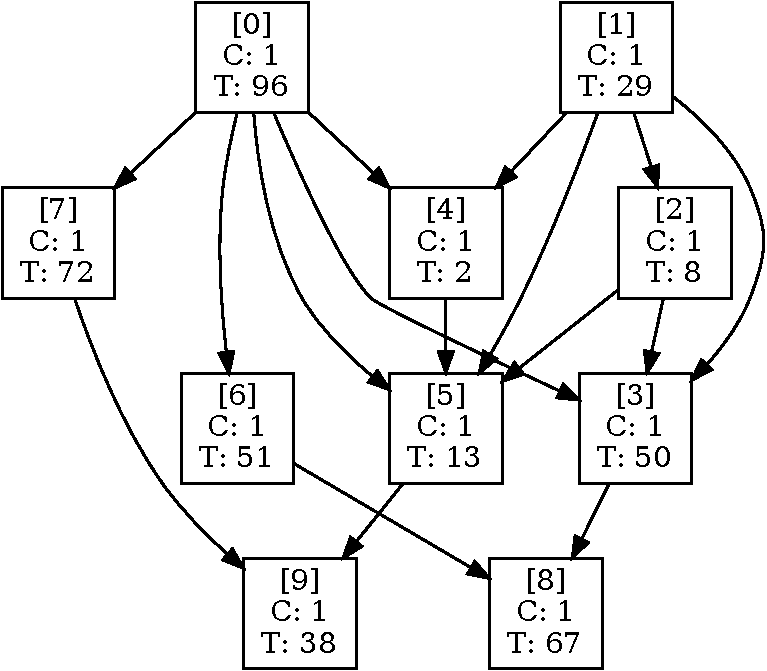
\includegraphics[keepaspectratio, width = \linewidth]{./src/figure/case_study_all_timer/u_0.05.pdf}}
            \hspace{3.0cm} Number of nodes: 10,\\ Total utilization: 0.05
        \end{minipage}
        % 3
        \begin{minipage}{0.45\linewidth}
            \centering
            \scalebox{0.58}{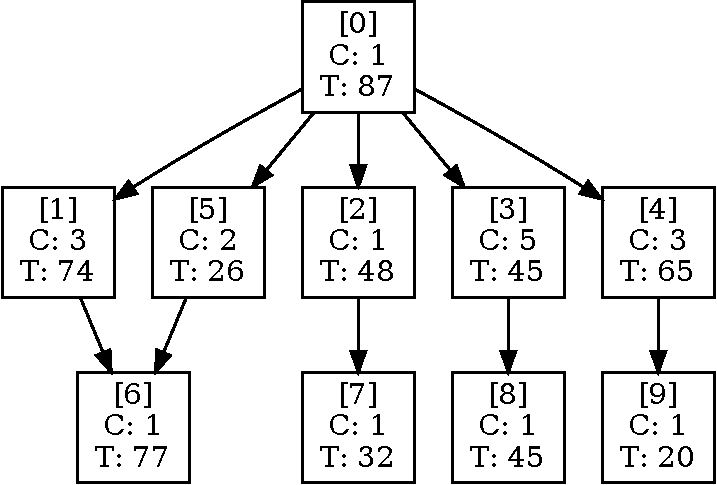
\includegraphics[keepaspectratio, width = \linewidth]{./src/figure/case_study_all_timer/u_0.5.pdf}}
            \hspace{3.5cm} Number of nodes: 10, Total utilization: 0.5 \\
            \vspace{3mm}
            \centering
            \scalebox{0.75}{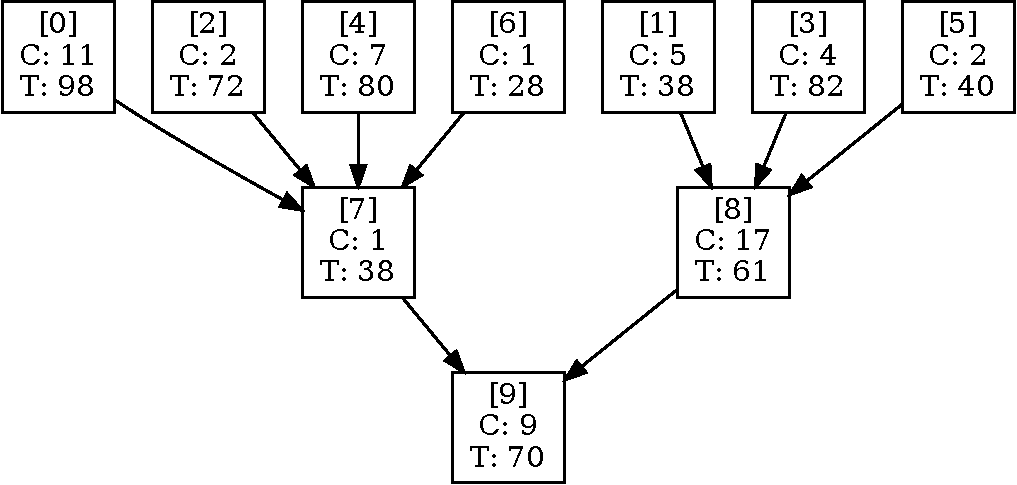
\includegraphics[keepaspectratio, width = \linewidth]{./src/figure/case_study_all_timer/u_0.95.pdf}}
            \hspace{3.0cm} Number of nodes: 10, Total utilization: 0.95
        \end{minipage}
    \end{tabular}
    \centering
    \caption{Example of generating multi-rate DAGs consisting of only timer-driven nodes of various total utilization.}
    \label{fig: case_study_all_timer}
\end{figure*}


Since CCR changes the nature of DAGs and affects the performance of scheduling algorithms, existing studies of single-rate DAGs have used random DAG sets with different CCR values in their evaluations.
An example of the generation in RD-Gen of a random DAG set with varying CCR, number of nodes, execution time, and communication time using the {\it Fan-in/Fan-out} method as used in existing studies \cite{subbaraj2020multi, liu2016minimizing, sheikh2016sixteen} is shown in Fig.~\ref{fig: case_study_single}.
Because the {\it Combination} is specified for the {\it Number of nodes} (lines 6-7 in Fig.~\ref{fig: case_study_single}) and {\it CCR} (lines 21-22 in Fig.~\ref{fig: case_study_single}), RD-Gen generates 100 random DAGs each for all combinations of these parameters (i.e., $\{10, 20, 30, ..., 1,000\} \times \{0.1, 0.2, 0.5, 1.0, 2.0, 5.0, 10.0\}$).
For each DAG, after graph construction, execution time is randomly assigned to each node in the range of 1 to 30 (lines 19-20 in Fig.~\ref{fig: case_study_single}).
Then, the total communication time is calculated from the CCR and the sum of execution time based on Eq.~(\ref{eq: ccr}), and the total communication time is randomly distributed to each edge.
Thus, the user can generate all DAG sets used in the evaluation with a single command, without adjusting the number of nodes and CCR.


\subsection{Case study 2}
\label{ssec: case_study_2}


Random DAG sets with different total utilization are used in the evaluation of most studies considering multi-rate DAGs.
An example of generating a multi-rate DAG with a random period and execution time for each node based on the total utilization of the DAG, as used in existing studies \cite{he2021response, gunzel2021suspension, ueter2021hard}, is shown in Fig.~\ref{fig: case_study_all_timer}.
Here, timer-driven nodes are drawn as squares.
Because {\it Combination} is specified for {\it Total utilization} (lines 21-22 in Fig.~\ref{fig: case_study_all_timer}), RD-Gen generates 100 DAGs each with total utilization from 5\% to 95\% in 5\% increments.
For each DAG, the utilization of each node is determined by the UUniFast method to satisfy the total utilization, and the execution time is calculated from the utilization and a randomly selected period from a uniform distribution ranging from 1 to 100.


\subsection{Case study 3}
\label{ssec: case_study_3}


\begin{figure*}[t]
    \begin{tabular}{c}
        %1
        \begin{minipage}{0.25\linewidth}
            \begin{flushleft}
                \begin{tabular}{l}
                    \lstset{linewidth=4.5cm, basicstyle=\scriptsize}
                    \lstinputlisting{src/code/case_study_chain.txt}
                \end{tabular}
            \end{flushleft}
            \centering
            Input YAML file
        \end{minipage}
        % 2
        \begin{minipage}{0.32\linewidth}
            \centering
            \scalebox{0.7}{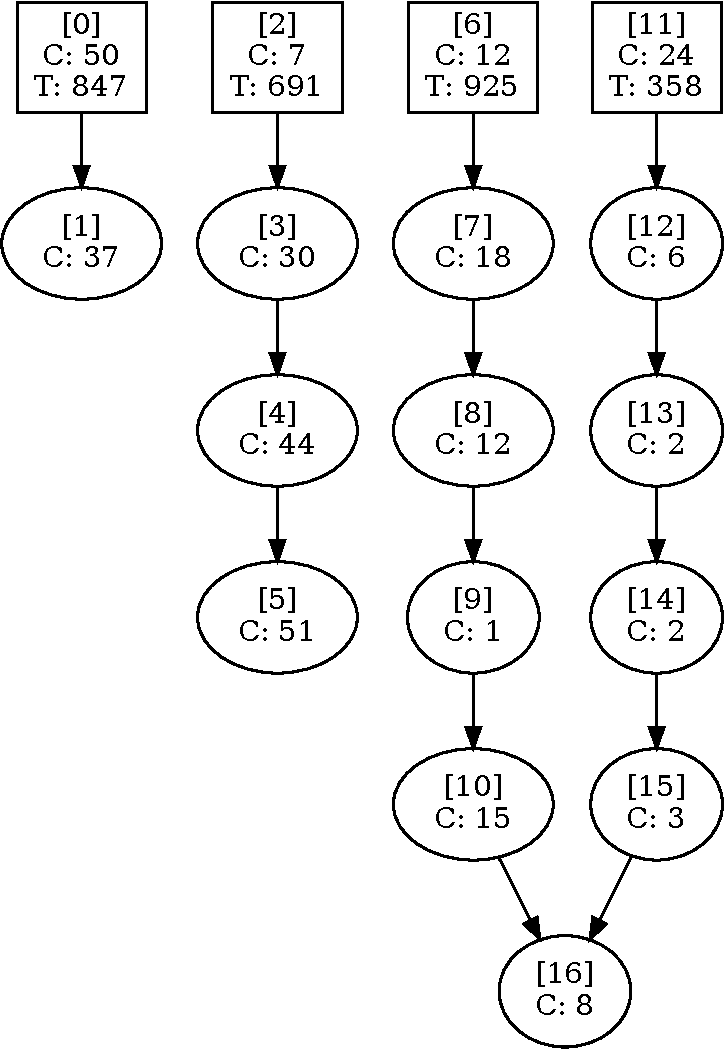
\includegraphics[keepaspectratio, width = \linewidth]{./src/figure/case_study_chain/u_0.5.pdf}}
            \hspace{3.0cm} Number of chains: 4,\\ Total utilization: 0.5, \\ Number of exit nodes: 3
        \end{minipage}
        % 3
        \begin{minipage}{0.36\linewidth}
            \centering
            \scalebox{1.0}{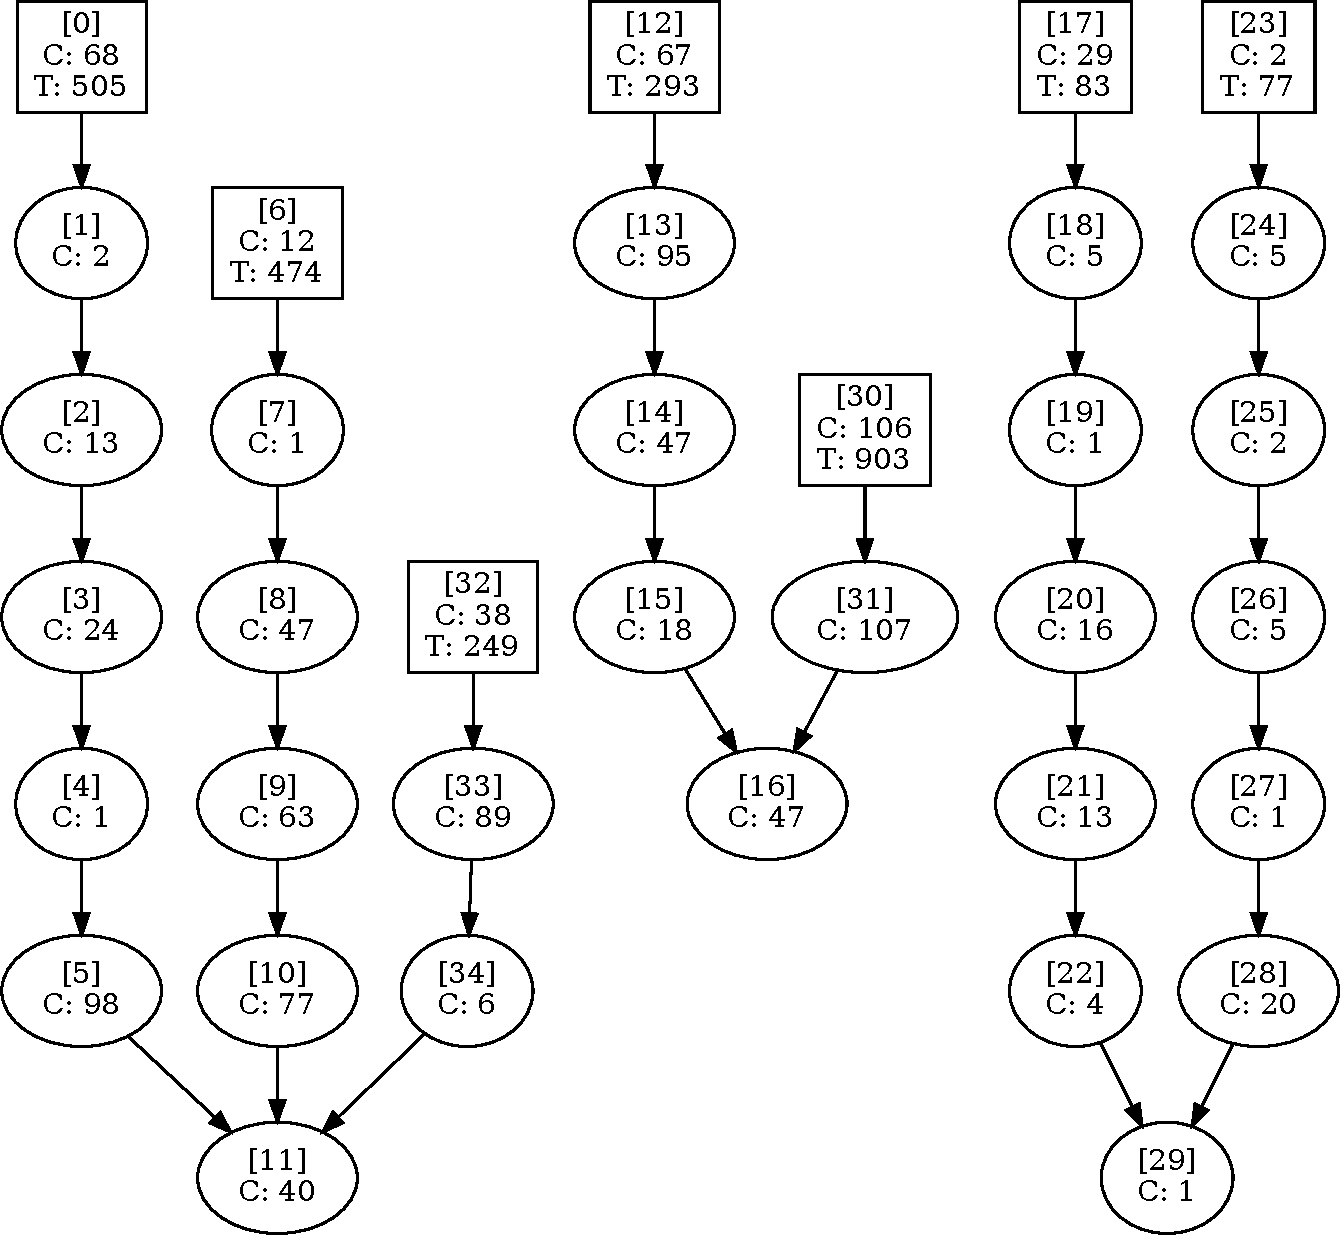
\includegraphics[keepaspectratio, width = \linewidth]{./src/figure/case_study_chain/u_4.0.pdf}}
            \hspace{3.5cm} Number of chains: 7, Total utilization: 4.0 \\ Number of exit nodes: 3
        \end{minipage}
    \end{tabular}
    \centering
    \caption{Example of generating chain-based multi-rate DAGs of various total utilization.}
    \label{fig: case_study_chain}
\end{figure*}


In the evaluation of chain-based multi-rate DAGs, a random DAG set is used with varying total utilization for the entire system and each chain.
An example of generating a random DAG set, as used in existing studies \cite{tang2020response, choi2021picas}, in which the utilization of each chain is determined from the total utilization of the entire system, and the chain period and execution time of each node is randomly assigned to satisfy the utilization of the chain is shown in Fig.~\ref{fig: case_study_chain}.
RD-Gen randomly sets the utilization of each chain using the UUniFast method to achieve a determined total utilization.
Here, since {\it Maximum utilization} is specified as 1.0 (line 24 in Fig.~\ref{fig: case_study_chain}), RD-Gen never generates a chain with a utilization greater than 1.0.
The period of each chain is randomly set in the range of 50 to 1${,}$000, and the execution time of each node is calculated based on the utilization and period (lines 10-18 in Algorithm~\ref{alg: set_utilization}).
